\chapter{Simple Network Management Protocol}\label{ch:snmp}
Large networks has too many components to be managed by human agents alone. Network devices have to maintain a large amount of management data such as configuration information,  operational state and statistics. Management information can be used to understand how a network performs, how devices in a network are configured and to change their configuration. The Simple Network Management Protocol (SNMP) \cite{rfc3410} is an application layer protocol that facilitates the exchange of management information between network devices. It exposes management data in the form of variables on the managed systems, which describe the system configuration. Since its first publication in 1988, the SNMP protocol has become the most widely-used network management tool for IP-based networks.

Currently, there are three versions of SNMP defined. The first version (SNMPv1) is nowadays a historical IETF standard, although it is still widely supported by many vendors. SNMPv1 has been criticized for its poor security based on a community string, which is a type of password transmitted in cleartext. SNMPv2 extended the functionality of SNMPv1 and includes a number of improvements, such as additional protocol operations. A new security system was proposed, however, it was too complex and was not widely accepted. SNMPv3 addresses the security problems of the previous versions. The SNMPv3 architecture introduces a well defined extensible architecture and the User-based Security Model (USM) for message security.

The SNMP protocol is datagram-oriented and its implementation can be very lightweight \cite{draft-6lowpan-snmp}. It can fit resource-constrained devices very well. This makes it a perfect candidate as a management protocol for 6LoWPAN applications. In this chapter an overview of the SNMP protocol is given.

\section{Protocol Architecture}
The SNMP protocol is designed to have a modular architecture, which allows the evolution of the protocol and enables protocol extensions. The architecture includes several subsystems communicating via defined abstract service interfaces. Abstract service interfaces describe the conceptual interfaces between various subsystems.  While the subsystems can be changed and extended over time, the interfaces are fixed.

\begin{figure}[htp]	
\begin{center}
    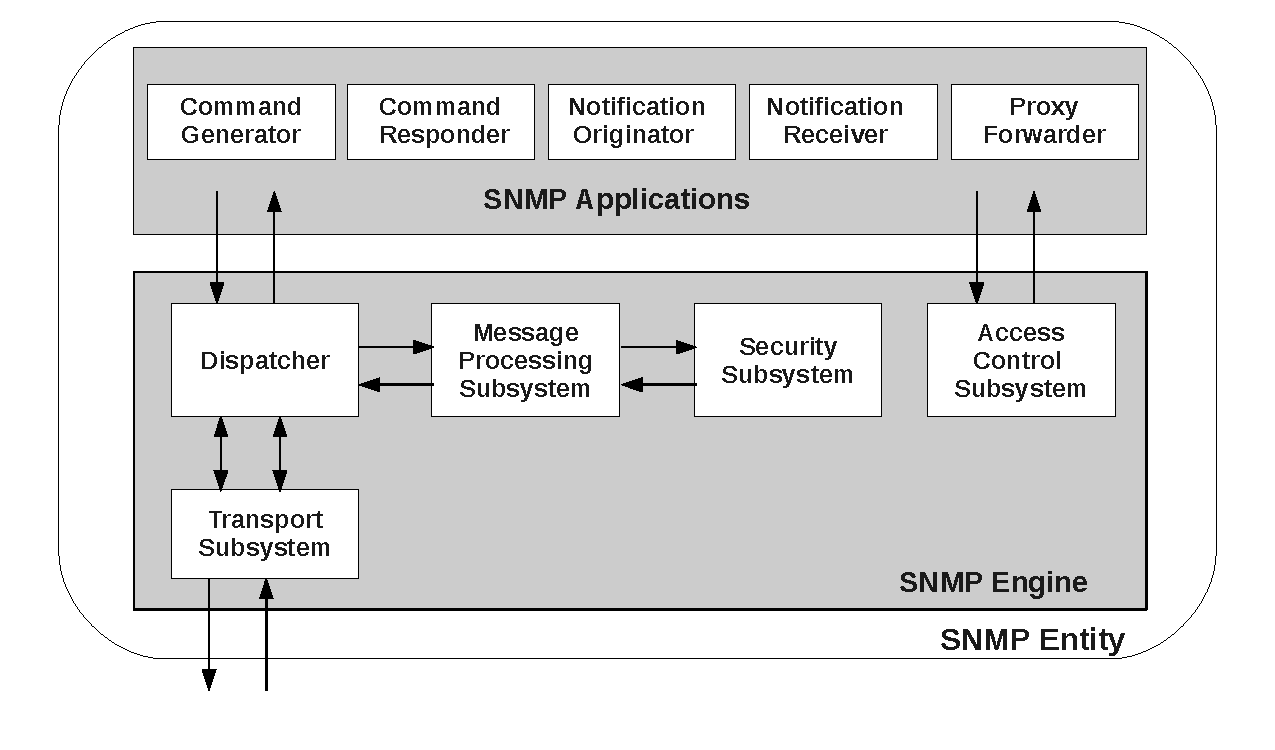
\includegraphics[scale = 0.6]{img/snmp-arch.pdf}
    \caption{Structure of an SNMP entity}   
	\label{fig:snmparch}
\end{center}
\end{figure}

According to the SNMP architecture defined in \cite{rfc3411}, an SNMP entity consists of an SNMP engine and one or more associated applications. The SNMP engine contains  a dispatcher, a message processing subsystem, a security subsystem, an access control subsystem, and a transport subsystem (Figure \ref{fig:snmparch}). Each subsystem may include multiple concrete models implementing different services. The dispatcher is responsible for controlling the data flow within an SNMP entity. Extracting data from received messages and preparing messages for sending are accomplished in the message processing subsystem. Each message processing model defines the format of a particular version of an SNMP message. Typically, the message processing subsystem supports three models for SNMPv1, SNMPv2c, and SNMPv3. The security subsystem provides security services such as authentication and privacy of messages. Authorization services are provided by the access control subsystem. The transport subsystem \cite{rfc5590} allows for multiple transport protocols to be used.

There are several types of defined applications (Figure \ref{fig:snmparch}), such as a command generator which monitor and manipulate management data, a command responder providing access to management data, a notification originator initiating asynchronous messages, a notification receiver processing these messages, and a proxy forwarder which forwards messages between entities. Applications may use the services provided by the SNMP engine. An SNMP entity which includes one or more command generator and notification receiver applications is called an SNMP manager. An entity containing one or more command generator and notification receiver applications is called an SNMP manager.


\section{Operations}

\section{Security Models}

